%% -*- coding: utf-8 -*-
%% Timestamp: "2025-05-05 12:50:00 (ywatanabe)"
%% File: "/home/ywatanabe/proj/SciTex/manuscript/src/figures/src/Figure_ID_02_architecture.tex"

% This is an example figure file showing the SciTex architecture.
% It demonstrates how to create more complex figures with multiple panels.

\begin{figure}[ht!]
    \centering
    
    % For this example, we'll create a simple diagram using TikZ
    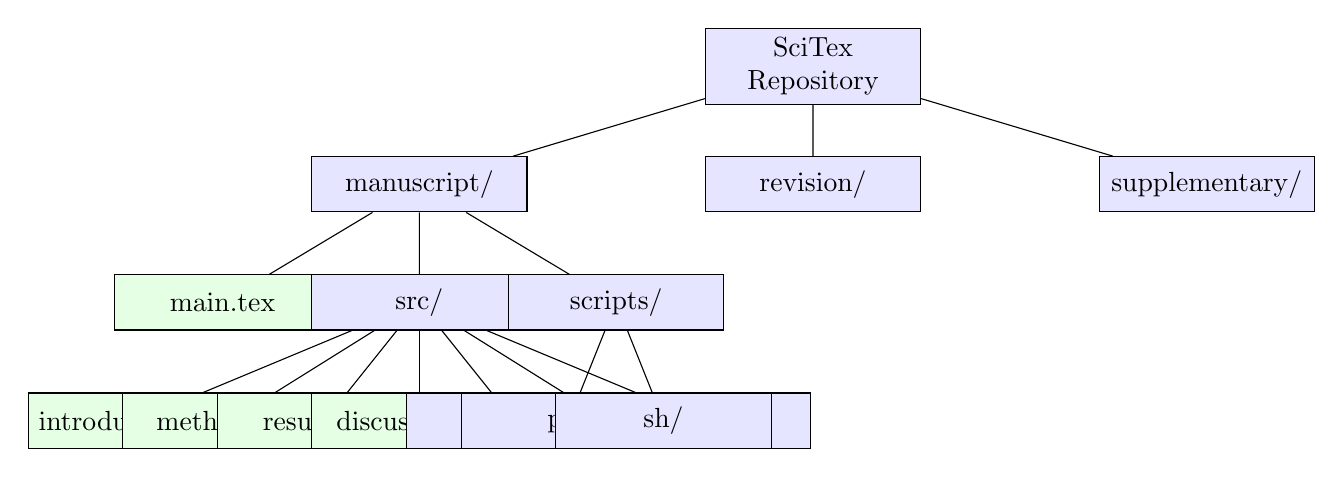
\begin{tikzpicture}[
        file/.style={rectangle, draw, fill=green!10, 
                     text width=2.5cm, text centered, minimum height=0.7cm},
        directory/.style={rectangle, draw, fill=blue!10, 
                     text width=2.5cm, text centered, minimum height=0.7cm},
        arrow/.style={draw, -latex, thick},
        level 1/.style={sibling distance=5cm},
        level 2/.style={sibling distance=2.5cm},
        level 3/.style={sibling distance=1.2cm}
    ]
    
    % Draw a hierarchical tree of the SciTex architecture
    \node[directory] (root) {SciTex Repository}
        child[level 1] {
            node[directory] (manuscript) {manuscript/}
            child[level 2] {
                node[file] {main.tex}
            }
            child[level 2] {
                node[directory] {src/}
                child[level 3] { node[file] {introduction.tex} }
                child[level 3] { node[file] {methods.tex} }
                child[level 3] { node[file] {results.tex} }
                child[level 3] { node[file] {discussion.tex} }
                child[level 3] { node[directory] {figures/} }
                child[level 3] { node[directory] {tables/} }
                child[level 3] { node[directory] {styles/} }
            }
            child[level 2] {
                node[directory] {scripts/}
                child[level 3] { node[directory] {py/} }
                child[level 3] { node[directory] {sh/} }
            }
        }
        child[level 1] {
            node[directory] (revision) {revision/}
        }
        child[level 1] {
            node[directory] (supplementary) {supplementary/}
        };
    
    \end{tikzpicture}
    
    \caption{\textbf{SciTex template architecture.} The figure shows the hierarchical organization of the SciTex repository, with emphasis on the manuscript component. The modular structure separates content files (introduction, methods, results, discussion), supporting materials (figures, tables), styling definitions, and automation scripts. This organization facilitates collaboration, version control, and maintenance of complex documents.}
    \label{fig:architecture}
\end{figure}

%%%% EOF